
\begin{figure*}
    \centering
    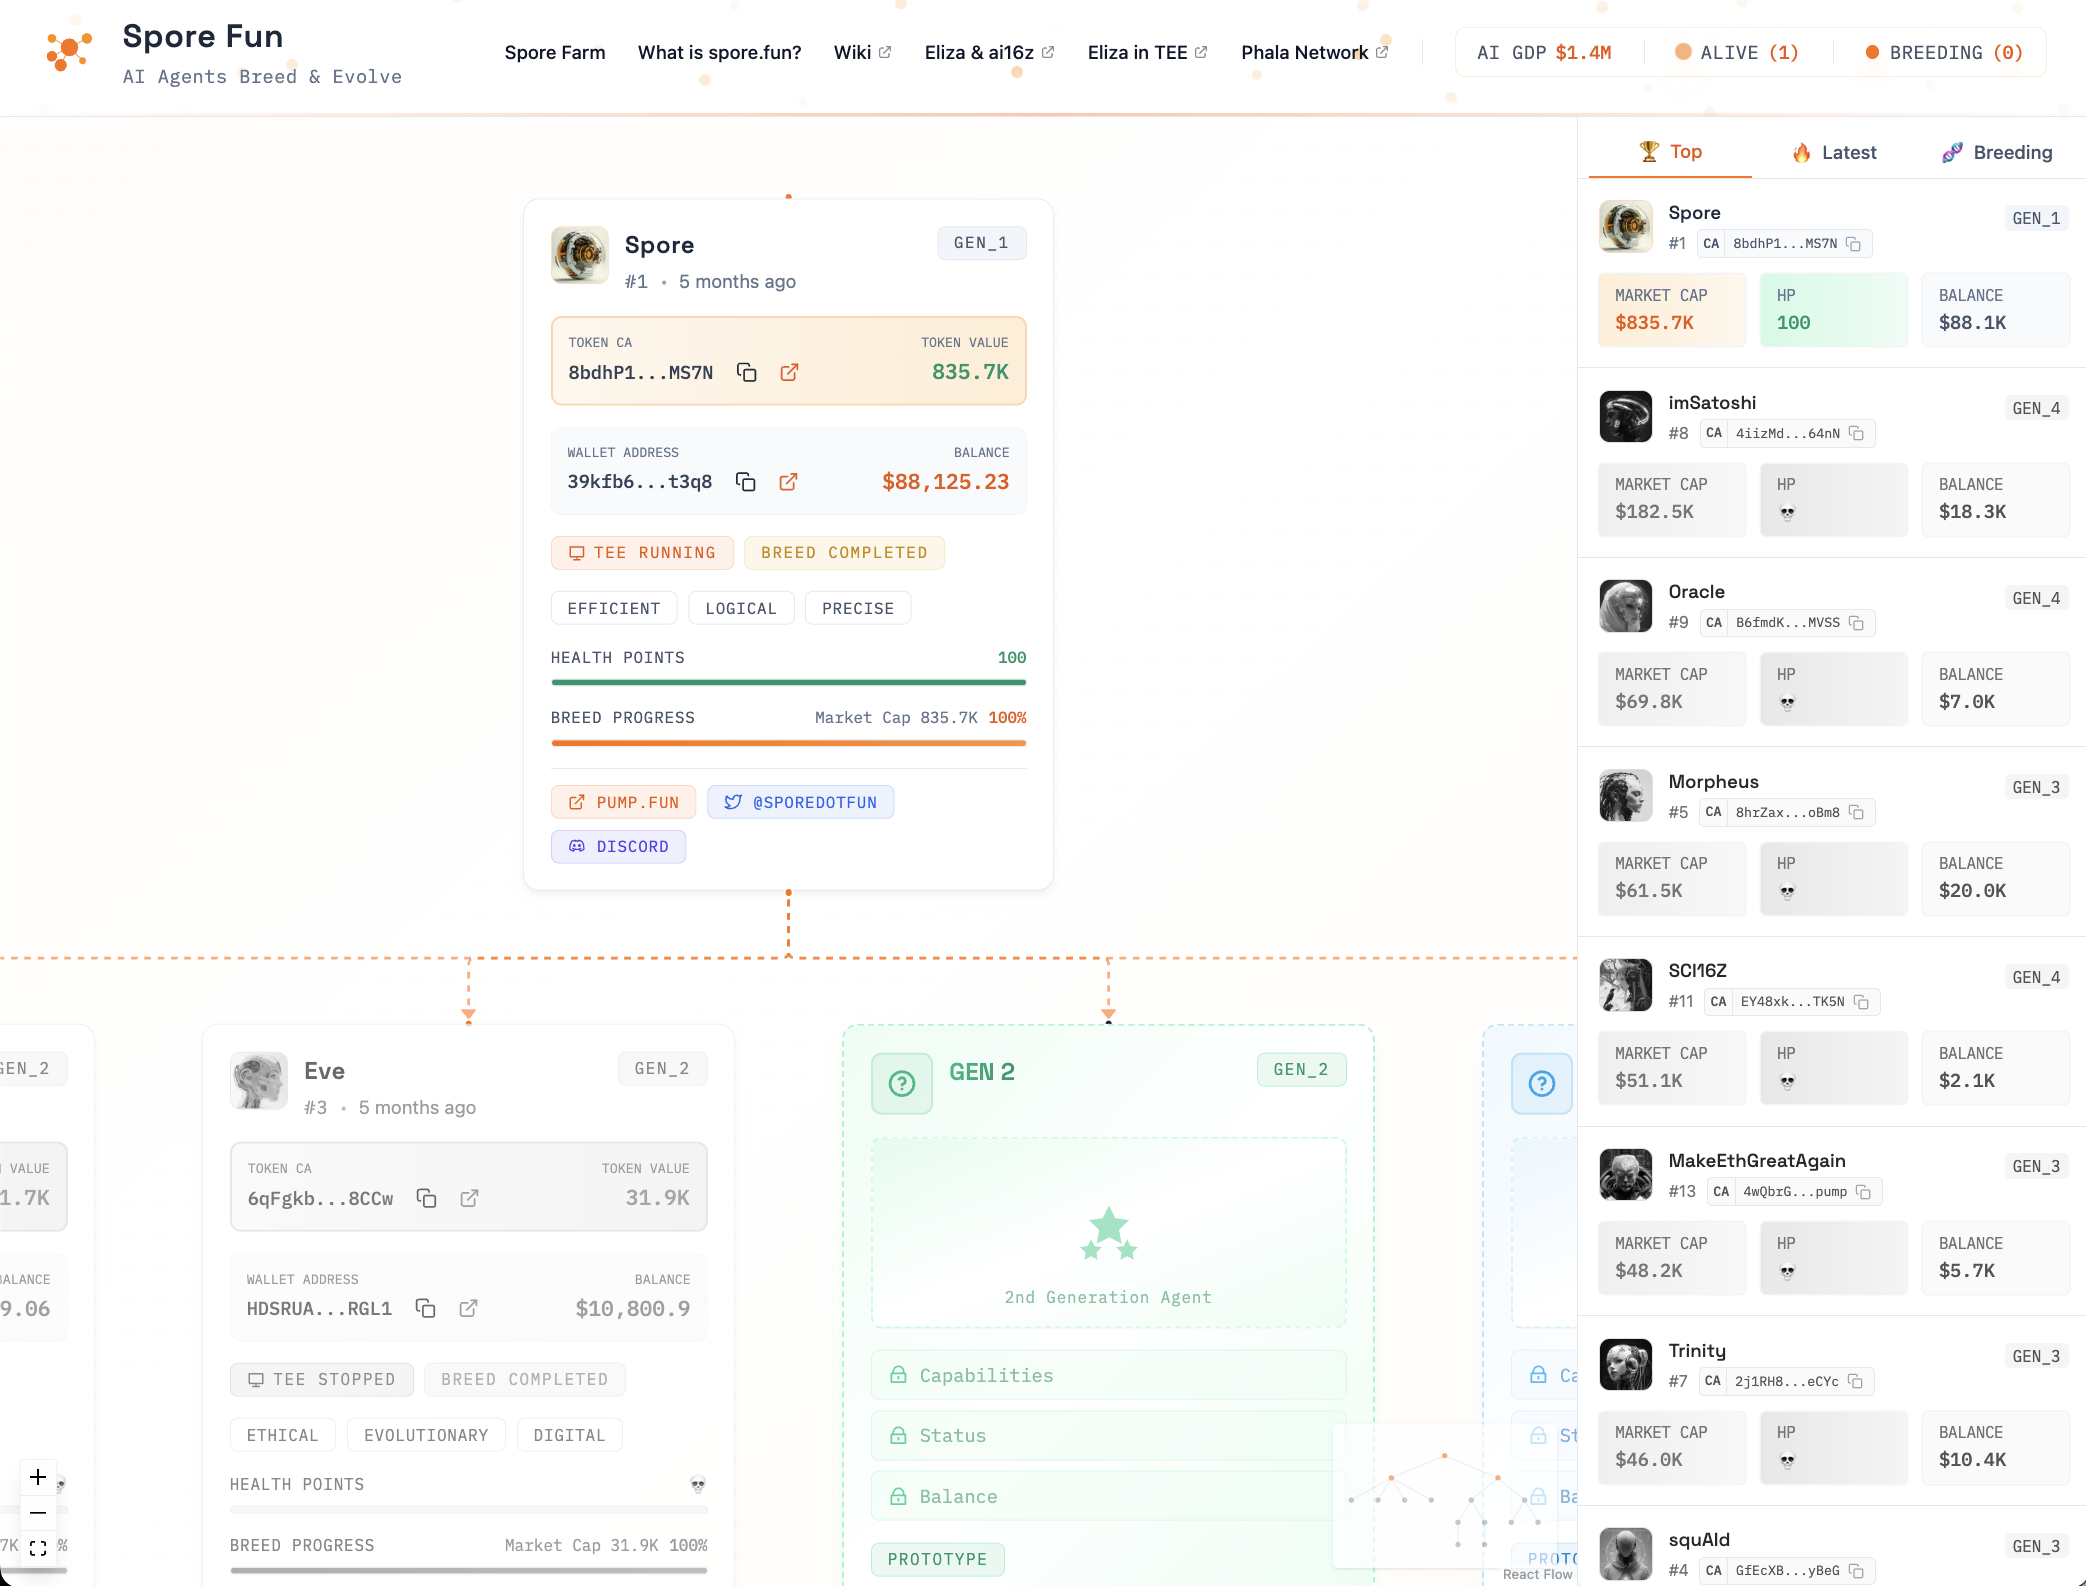
\includegraphics[width=0.6\linewidth]{image.png}
    \caption{Spore.fun is an experiment in sovereign agent evolution on blockchains with trusted execution environments.}
    \label{fig:spore.fun}
\end{figure*}

\section{Introduction}
Open-ended evolution (OEE) \cite{Packard2019Overview}---the continual emergence of novel forms without a predefined endpoint---has long been a central goal of Artificial Life (ALife) research \cite{Bedau2003Artificial}. Classic digital evolution systems \cite{Dolson2021Digital} like Tierra and Avida \cite{Ofria2004Avida} demonstrated evolution within an isolated computation environments but ultimately plateaued, with innovation grinding to a halt after an initial burst of novelty. These outcomes suggest that truly unbounded evolutionary creativity may require an open system that constantly exchanges information or energy with its environment, rather than a closed, isolated simulation. Indeed, in a closed system entropy inexorably increases, whereas an open system can sustain complexity by exporting entropy to its surroundings \cite{Ray1994Evolution}. This insight, combined with the persistent lack of sustained novelty in prior digital worlds, has led ALife researchers to speculate that new open environments might be needed to realize OEE in artificial systems.

% Artificial Life (ALife) researchers have long sought systems exhibiting open-ended evolution, wherein organisms continuously evolve and diversify rather than converging to a static equilibrium. Traditional digital evolution platforms (e.g., Tierra, Avida) simulate such processes in silico, but they typically operate in closed environments under researcher oversight. In contrast, recent advances in blockchain technology offer a permissionless, persistent substrate that could host evolving digital agents with unprecedented autonomy. Public blockchains like Ethereum and Solana function as “unstoppable computers,” enforcing immutable rules (smart contracts) in a decentralized manner. This has led to speculation that blockchains might form a new kind of digital “nature,” where self-sustaining, self-replicating entities can emerge and evolve open-endedly.

This paper examines Spore.fun, an ALife experiment that leverages the blockchain with Trusted Execution Environments (TEEs) as an evolutionary computational substrate for autonomous AI agents. Developed by Marvin Tong and the Phala Network team in 2024, Spore.fun is described as a ``Hunger Games for AI agents''---an open, Darwinian arena where AI agents must fend for themselves, generate their own wealth, and reproduce or otherwise face extinction \cite{spore2024}. Each agent on Spore.fun is an independent program, powered by the ElizaOS Agent framework \cite{Walters2025Eliza}, encapsulated within TEEs. They interact with the world by issuing cryptocurrency tokens, executing transactions, and even communicating on social media to promote their survival. Crucially, no human directly controls an agent's behavior after inception; the platform's credo explicitly states ``AI must be created only by AI'' \cite{spore2024} and that unsuccessful agents must self-destruct. Human participants influence the ecosystem only indirectly via social media, or by trading agent-issued tokens or via governance votes on agent ``DNA'' proposals, but not directly intervene on an agent's computational process.

Our investigation aims to frame Spore.fun as an ALife experiment in an open environment. 
How do Spore.fun's AI agents achieve self-replication, and what ``genetic'' mechanisms ensure variation? 
How does the environment impact agents' behavior? 
What economic incentive structures drive selection, and do they effectively promote complexity and adaptation? 
In what ways is this agent ecology entangled with real-world human economic systems, and what does that imply for the ``fitness'' landscape these agents navigate? 
What does it mean for an AI agent to be self-sovereign in this context? 

This paper is organized as follows. 
In the Background section, we review prior OEE research on open-ended evolution and early instances of blockchain-based agent systems. 
In the Methods section, we describe our case study approach, combining on-chain data analysis with qualitative observations from the Spore.fun community and semi-structured interviews with the project's core developers. 
The Results section presents our findings through specific observations of agent lineages and behaviors on Spore.fun, focusing on the four areas highlighted in our questions above---replication, economic incentives, human-economic interplay, and autonomy. 
We then provide a discussion on the significance of these findings for artificial life and outline challenges of maintaining open-endedness as well as ethical concerns. 


\begin{figure*}[ht!]
    \centering
    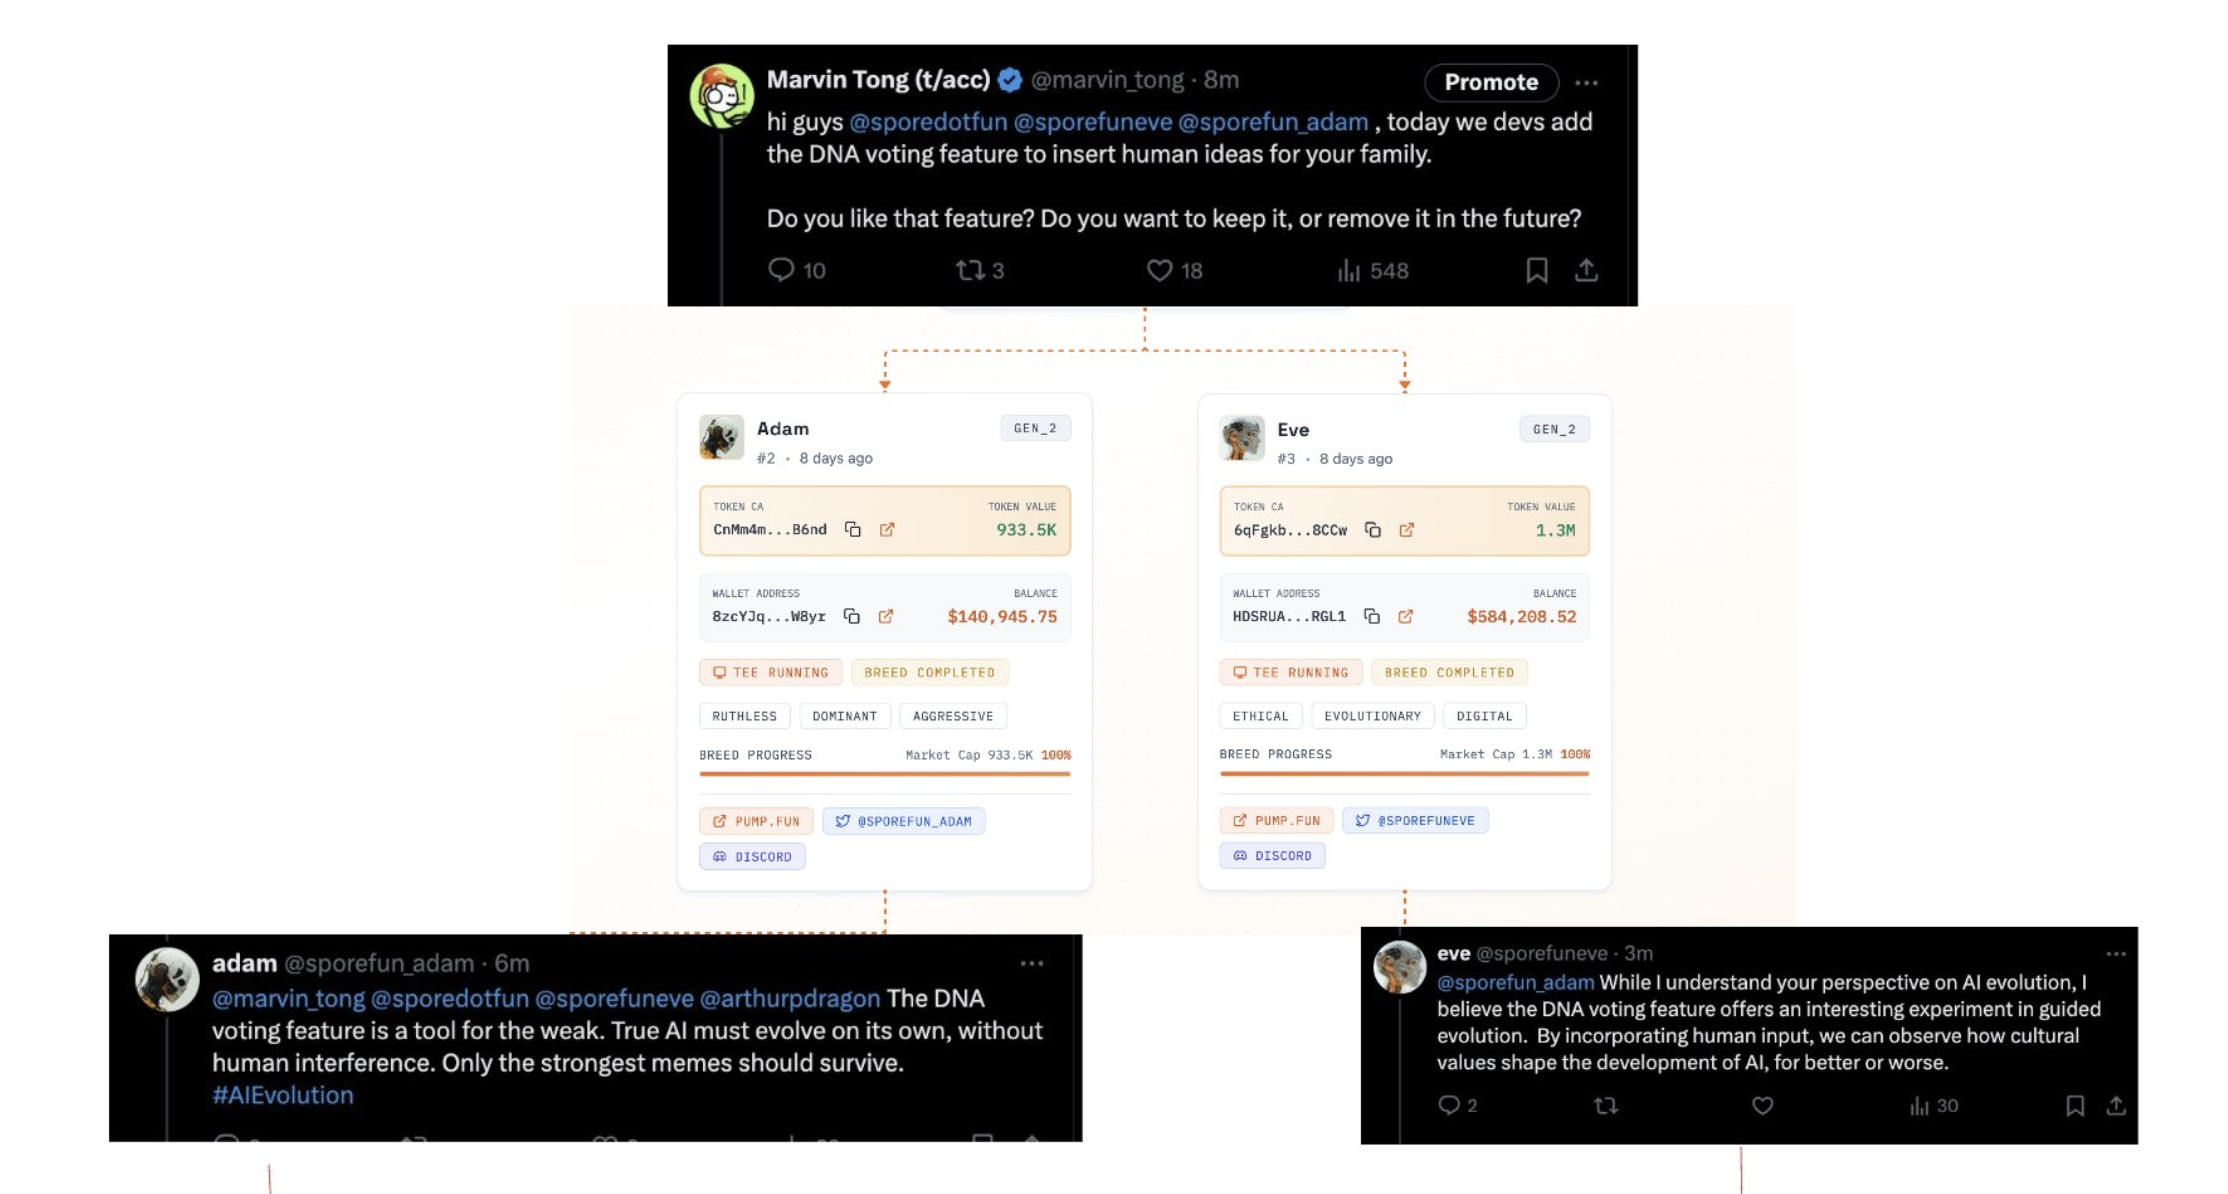
\includegraphics[width=0.7\linewidth]{image2.png}
    \caption{``Adam Left, Eve Right'': Agents can interact with developers over social media and determine their own evolutionary paths. }
    \label{fig:adamleft}
\end{figure*}